\chapter{Music as an embodied process}\label{chapter:music-cognition}

`It doesn't make sense to sit there and listen to this music; you need to get up and dance,' the woman said as she gently pushed my fellow students onto the dance floor. She was standing in a \emph{bunad}, a traditional Norwegian folk costume, in front of my group of first-year music students. We had been sent to the idyllic village of Voss in Western Norway for a one-week intensive course in folk music and dance. We all thought that we would spend most of the time playing and listening to music. As it turned out, the days were split equally between playing and dancing. We quickly discovered the embodied nature of the various Norwegian folk music traditions. You need to dance, to understand the asymmetrical triple meter of Telespringar tunes. Norwegian folk music is no more special than other folk musics. In most cultures there are close relationships between music and dance, what \citet{haugen_music-dance._2016} has called \emph{music--dance} to emphasize the connectedness. Some languages even only have one term to describe the shared activity of playing, dancing, and singing, such as the word `ngoma' in pro-Bantu linguistic-cultural groups  \citep{bjorkvold_muse_1992,sarath_redefining_2016}. But the body is essential for the musical experience also when one is not dancing.


\section{The body in music}

Even though \citet{small_musicking:_1998} approached musicking from a sociocultural perspective, many of his reflections resonate well with an embodied approach to understanding the experience of music. This can be seen in his analysis of the strict behavioral `laws' imposed on both performers and perceivers in the classical concert hall. In such a setting, the audience is expected to sit quietly, with as little motion and emotional expression as possible. Even with such rules suppressing the body and its motion, Western art music concerts are also embodied. There are numerous references to body motion in sheet music, such as metaphors like \emph{staccato}, \emph{ritardando}, and \emph{lento}. Such motion qualities embedded in the scores can probably be traced back to the composer's imagined sensations of bodily activity. These imagined motion qualities may (or may not) be interpreted in the performed music through the performer's actions and may, in turn, also lead to physical motion in the perceivers. So even in score-based music, there are close connections between body and mind. Many other musics---and notably different types of dance music---are created with motion as a core element.

Given the apparent importance of the body for both music performance and perception, it is strange that it was only relatively recently that the study of the body's role in music took off. In 20th-century musicology, relatively little attention was devoted to the topic, even though several people argued for its inclusion, such as \citet[vii]{clynes_music_1982}:

\begin{quote}
There is much music in our lives --- yet we know little about its function. [\ldots] [T]he coming years are likely to see much progress towards providing answers and raising new questions. These questions are different from those music theorists have asked themselves: they deal not with the structure of a musical \emph{score} [\ldots] but with music in the flesh: music not outside of man to be looked at from written symbols, but music-man as a living entity or system.
\end{quote}

Clynes' reflection was a response to a more general trend in psychology and cognitive science, which has later led to the development of what is nowadays often called \emph{embodied cognition}.


\section{Embodied cognition}

An embodied approach to cognition may be seen as an opposition to a traditional cognitive view of the body and mind as separate entities \citep{shapiro_embodied_2019}. Standard cognitive theories are based on the idea of the brain as a `device' that passively receives inputs from the world, processes them, and outputs responses. On the other hand, embodied cognition takes the body and its perceptual and motor capacities as having a fundamental role in understanding how we experience the world. This not only relates to how we interact with our surroundings. The interaction is also the basis for creating \emph{meaning} in the world. From an embodied perspective, meaning is not based on abstract concepts and ideas, but rather something that we create through our bodily interactions in the world  \citep{dourish_where_2001}.

One of the core elements of embodied cognition is the close relationship between action and perception: the \emph{action--perception loop}. \citet{hurley_consciousness_1998} refers to cognition as a `sandwich' of action and perception (Figure~\ref{fig:cognition1}). The idea here is that perception is not based on the passive reception of external stimuli; perception guides one's actions. Or, in the words of \citet[p. 1]{noe_action_2004}:

\begin{quotation}
Perception is not something that happens to us, or in us. It is something we do.
\end{quotation}

\begin{figure}[tp]
\centerline{
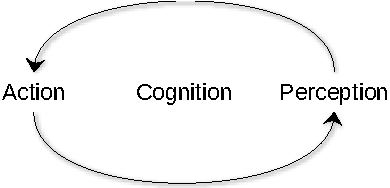
\includegraphics[width=.5\columnwidth]{figures/12-sandwich-crop.pdf}
\caption{A sketch of what \citet{hurley_consciousness_1998} called the cognition `sandwich.'}
\label{fig:cognition1}
}
\end{figure}

\citet{noe_action_2004} exemplifies how such an action--perception loop works in real-life by referring to a blind person moving around a room with a stick. The active tapping with the stick helps discover the space by listening to the sonic responses from the tapped objects and the room's acoustic properties. Blind people often develop a sharp auditory sense, but the same principles are also used by seeing people. If I move my head, I will see something different than if I look straight ahead. If I walk to a different location, I will hear something else than in my current location. As such, the action--perception loop is bi-directional; perception predicts action, and action predicts perception \citep{schutz-bosbach_perceptual_2007}.

In his ecological psychology, \citet[p.222]{gibson_ecological_1979} stresses the importance of a person's relationship with the \emph{environment}:

\begin{quotation}
One sees the environment not just with the eyes but with the eyes in the head on the shoulders of a body that gets about.
\end{quotation}

The environment should here be understood as anything external to the person in question. It includes the physical space one is within but also objects and other people. Figure~\ref{fig:cognition3} illustrates this by sketching the constant interaction between the body, the mind, and the environment. There are still many holes in our understanding of how such interactions work in the brain. Current research tries to verify various proposed theories. One of these is the \emph{dynamic systems theory}, which suggests that we learn to live in the world through spontaneous self-organization in complex interactions between the body and the environment \citep{lorenz_deterministic_1963}. These interactions occur at different spatial scales and at multiple time scales. According to the \emph{theory of neuronal group selection}, the brain starts early in life with a primary neuronal `repertoire' \citep{edelman_neural_1987}. New neuronal combinations are constantly formed, and the combinations that provide the best `solutions' are strengthened and further developed.

\begin{figure}[tp]
\centerline{
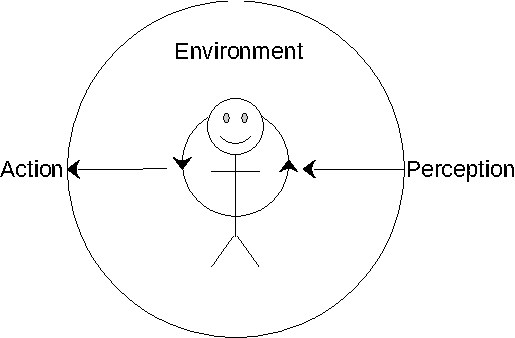
\includegraphics[width=.7\columnwidth]{figures/13-gibson-crop.pdf}
\caption{A sketch of an `internal' loop between mind and body and an `external' loop between body and environment.}
\label{fig:cognition3}
}
\end{figure}

The three theories mentioned above---the action--perception loop, the dynamic systems theory, and the theory of neuronal group selection---can be seen as complementary. The action--perception theory describes interactions between an individual and the environment. The dynamic systems theory explains how movement patterns change depending on context. The theory of neuronal group selection describes how the neuronal system adapts to changing stimuli. As such, all the theories acknowledge that the world is complex and that our interaction with the world is based on tackling this complexity by continuously adapting our behavior. The theories are also based on the idea that there can be multiple ways of handling a problem. That is why we can perform actions, say moving a chair, in many different ways. Such a flexible approach to living is learned through childhood, and the interactions are developed as we get older and acquire more skills.


\section{Embodied music cognition}

In the book \emph{Ways of Listening}, \citet{clarke_ways_2005} suggests that an embodied approach to music perception should be based on \emph{ecological listening}. This involves taking our everyday listening and our auditory system's capacities as the point of departure for understanding meaning in music. A large part of our continuous listening is concerned with discriminating between different sound events, what \citet{bregman_auditory_1994} calls \emph{auditory scene analysis}. Through evolution, we have adjusted our hearing to what is presumably crucial for our survival. Clarke argues this evolutionary developed auditory system is the basis for composing, performing, and perceiving music. Thus, our perception of musical sound should be studied regarding our auditory system's capacities and limitations.

In his book, Clarke explains how we approach new sonic/musical material through three reasoning steps. The first level is about identifying `what sounds are the sounds \emph{of}, and what to do about them' \citep[p.3]{clarke_ways_2005}.
Such `sonic causality' can be seen as identifying which objects are involved in the sound production. The second level of listening is connected to the meaning gained when you understand what a sound is the sound of. The third level is related to how the sounds layer and interact with each other. We usually explore many sounds simultaneously, and what could be considered `foreground' sounds are also being merged into sounds of the `background.'

What differentiates the ecological listening theory of \citet{clarke_ways_2005} from more traditional music psychological approaches is the inclusion of culture in the discussion. This is illustrated in an analysis of Jimi Hendrix's performance of the Star-Spangled Banner at Woodstock in 1969. The meaning(s) attached to this performance---and its impact---needs to be understood as a complex interplay between the cultural contexts that the performance happened within and the musical features. Clarke convincingly shows how an interpretative musicological analysis can be combined with a cognitive framework.

One limitation of Clarke's approach in \emph{Ways of Listening}, which he acknowledges early on in the book, is the primary focus on sound. While his argument is certainly based on the idea that listening to sound is a multimodal phenomenon, he does not develop his argument into a fully embodied approach. This is what \citet{leman_embodied_2008} tries to do in his book \emph{Embodied music cognition and mediation technology}. Here, he sets out to create a complete model of musical communication, as sketched in Figure~\ref{fig:cognition6}. Musical intentionality is at the model's core, and Leman argues that a performer's intentions are only indirectly communicated. Direct communication is based on auditory and visual cues. As such, the performer's actions are overt representations of covert intentionality.

\begin{figure}[tp]
\centerline{
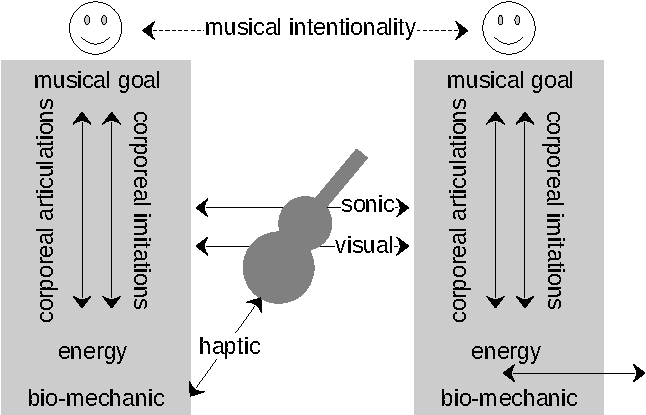
\includegraphics[width=0.8\columnwidth]{figures/14-leman-model-crop.pdf}
\caption{A model of embodied music cognition, based on \citep[p.160]{leman_embodied_2008} (see text for explanation).}
\label{fig:cognition6}
}
\end{figure}

In Leman's model, the action--perception loop is represented through an internal loop between \emph{corporeal} articulations and imitations. What happens in the body is mirrored in the brain. Similarly,  what happens in the brain is the starting point for further actions.
This is not limited to performers. Perceivers also have an ongoing internal loop between mind and body. This may be why we have an urge to move when listening to music or get physical sensations when seeing other people play an instrument.

Leman describes the performer's multisensory interaction with the instrument, including auditory and visual feedback and haptic stimuli. The perceiver only sees/hears the auditory and visual stimuli but does not get any haptic stimuli from the instrument. However, based on previous haptic experiences and an internal loop between mind and body, one can speculate that a perceiver gets a sense of the haptic feedback by only listening/seeing a performance. For example, when I watch someone play the guitar, I can `feel' how it is to touch the strings. This type of sensation I can get by only imagining someone playing the guitar. It is precisely this type of complex loops between the minds and bodies of both performers and perceivers that Leman's model tries to explain.


\section{Motor-mimesis}

When it comes to our mental representations of music, or what could be called \emph{musical imagery}, \citet[p.318]{godoy_motor-mimetic_2003} has suggested that these may be based on \emph{motor-mimetic} principles:

\begin{quotation}
Motor-mimesis translates from musical sound to visual images by a simulation of sound-producing actions, both of singular sounds and of more complex musical phrases and textures, forming motor programs that re-code and help store musical sound in our minds.
\end{quotation}

This builds on the \emph{motor theory of perception}, which was proposed in linguistics to explain the close connections between action and sound in speech perception  \citep{liberman_motor_1985}. Here the claim is that language perception and acquisition are based on learning the `articulatory gestures' of the human vocal apparatus. Such articulatory gestures can be seen as the basic `atoms' out of which phonological structures are formed \citep{browman_articulatory_1989}. The motor theory of perception further postulates that the phonological, lexical, and syntactic structures are based on neural systems that have evolved for general motor control. This implies that the perceptual mechanisms of the vocal apparatus were in place long before language entered the stage and that speech and language adapted to phylogenetically older structures rather than the other way around \citep{lindblom_status_1991}.

The motor theory of perception received renewed interest after \citet{gallese_action_1996} found \emph{mirror neurons} in monkeys' brains. These experiments showed that a particular set of neurons were activated both when a monkey performed a goal-directed action and when observing another monkey performing a similar action. These and later experimental results support the idea that we continually simulate the actions we see. Such a mental `replay' of actions probably helps to learn. It may also explain our ability to make predictions. \citet{wilson_case_2005} argue that we continuously simulate our actions in parallel to the physical actions carried out. Such imitative motor activation feeds back into the perceptual processing and allows us to adjust our actions accordingly.

The early experiments on mirror neurons were of goal-directed actions observed in monkeys. Later, \citet{rizzolatti_language_1998} carried out positron emission tomography (PET) studies of humans and found that motor areas in the brain were activated during speech perception. Such an \emph{auditory-motor interaction} has also been shown in functional magnetic resonance imaging (fMRI) scans of humans \citep{hickok_auditorymotor_2003}. Here similar neuronal activity was found when subjects only listened to speech or music and covertly hummed the auditory stimuli.

Another set of studies has shown the existence of \emph{audiovisual mirror neurons} in the brain. This was found in experiments on monkeys, where the same neuronal response was measured whether the monkey could both see and hear a sound-producing action or only hear the sound of the same type of action \citep{kohler_hearing_2002}.
There have also been studies of audiovisual mirror neurons with more complex sounds. For example, \citet{haueisen_involuntary_2001} used magnetoencephalography (MEG) to show pianists' involuntary motor activity while listening to well-known piano music. \citet{lahav_action_2007} reported that similar motor activity might occur in non-musicians. They carried out an experiment during which non-musicians practiced playing a melody for a couple of weeks (learned by ear). After this practice, fMRI scans showed that motor areas in the brain were active when the subject listened to the same melody as had been practiced and when the person was not moving. This activation would only occur when listening to the same melody the person had practiced; variations on the melody resulted in little or no activation. This can be thought of as an `action-listening' process during which we continuously simulate the sound-producing actions related to the sounds we hear.

How does the discovery of mirror neurons, and the growing body of empirical evidence supporting the motor theory of perception, help develop the field of embodied music cognition? In his \emph{mimetic hypothesis}, \citet{cox_music_2016} proposes 20 principles for explaining musical experiences. His approach focuses on the perceiver and does not include the feedback loop between the performer and perceiver that we find in the model of \citet{leman_embodied_2008}. On the other hand, Cox digs deeper into the idea that perceivers experience music through embodied imitation of what he calls the `bodily motions and exertions' involved in producing music.
He also makes a distinction between \emph{overt} and \emph{covert} mimetic behavior. Overt behavior, such as moving the arm, he calls \emph{mimetic motor action} (MMA). Covert behavior is called \emph{mimetic motor imagery} (MMI), and is the experience of muscle tension without motion. Of his 20 principles \citep[p.13]{cox_music_2016}, some are of particular interest for my further argument:

\begin{itemize}

\item Principle 1: Sounds are produced by physical events; sounds indicate (signify) the physicality of their source.

\item Principle 2: Many or most musical sounds are evidence of the \emph{human} motor actions that produce them.

\item Principle 3: Humans understand other entities (animate or not, human or not) and events in their environment in part via mimetic behavior (MMI and MMA).

\item Principle 5: Mimetic comprehension is based on visual, auditory, and/or tactile information.

\item Principle 11: Any and all acoustic features can or will be mimetically represented.

\item Principle 12: Different kinds of music `invite' (motivate) different kinds of mimetic engagement, contributing to the feel (quale) of music.
\end{itemize}

The three first principles are similar to my thinking about action--sound couplings that we will get to in Chapter~\ref{chapter:couplings}. In the following will look more at two concepts from Principles 5 and 12: multimodality and affordance.


\section{Multimodality}

A fundamental aspect of embodied (music) cognition is that our perception is inherently \emph{multimodal}. This means that all our senses and modalities (as summarized in Table~\ref{table:senses}) are present when experiencing the world. That is why I prefer the term perceiver over listener. Many people say that they think about listening as a multimodal activity. However, I like to use a word that reminds me that all the senses are at work. Then it is also possible to reserve the term listening to the act of auditory perception.

\begin{table}[tbp]
\begin{center}
\caption{The human senses and their corresponding sensory organs and modalities \citep[p.5]{schomaker_taxonomy_1995}.}
\label{table:senses}
\begin{tabular}{l|l|l}
%\hline
Sensory perception  & Sensory organ & Modality 	\\
\hline
Sight         & Eyes		  & Visual 			\\
Hearing		    & Ears			& Auditory 		\\
Touch			    & Skin			& Tactile 		\\
Smell			    & Nose			& Olfactory 	\\
Taste			    & Tongue		& Gustatory 	\\
Balance		    & Organ of equilibrium 	& Vestibular 	\\
%\hline
\end{tabular}
\end{center}
\end{table}

One problem with using perceiver as a general term is that it may sound like the focus is only on the sensory input and not on the cognitive processes. One could argue that a word like `experiencer' could be better, but that may be a bit too broad again. For now, I have therefore decided to use perceiver as my primary term.

When I first started using perceiver instead of listener, it felt awkward, and I got many questions. After using it for some years, it feels normal. It has been so internalized that I rarely think about it any longer. Someone once asked me if I did not mean `receiver' instead of `perceiver,' pointing out that the `reception of music' has been used in some musicology literature. My answer was that these are entirely different terms. I think that a receiver is the opposite of a perceiver. A model based on having a sender and a receiver signals unidirectional and passive communication. The embodied music cognition paradigm, on the other hand, is built around the idea of a continuous feedback loop between performer and perceiver.

The senses and modalities work in parallel, and they also mutually influence each other. Let us set up a thought experiment of the interdependence and inseparability of our modalities. Think about walking down the street, while suddenly you \emph{hear} the sound of a guitar being played. Most likely, you will \emph{turn} towards where the sound is coming from and \emph{see} who is playing. Already at this point, three modalities have been at work: the \emph{auditory}, the \emph{visual}, and the \emph{vestibular}. First, your hearing's omnidirectional nature recognizes the sound. Then you turn so that the directionally limited sight can see the location of the sound source. Here the vestibular modality is vital for keeping you in balance and informing you about the orientation and motion of your head and body. This seemingly simple example of an everyday musical experience shows some of the richness of our multimodal capacities.

An exciting aspect of our multimodal perception is that we rarely pay attention to which modality is at work, and it often does not matter. For example, think about how you recognize other people. This can be through hearing their voice, seeing their way of moving, smelling their perfume, or a combination of these. We rarely think about which senses are at work, even though we may choose to focus on one particular sense if we want to. The senses work together most of the time, helping us move around in a complex world with a continuous stream of perceptual input.

Our multimodal capacity may also give rise to \emph{crossmodal} behavior, such as in synaesthesia, sensory substitution, and crossmodal perception. The McGurk effect is a famous example of the latter. \citet{mcgurk_hearing_1976} carried out an experiment where the subjects heard the spoken word `Ba' while seeing the video of a mouth saying `Ga.' However, the subjects did not perceive any of these two words but saw/heard `Da,' a combination of the two stimuli. There have been attempts to find similar types of audiovisual integration in music. In a clarinet performance study, \citet{vines_cross-modal_2006} showed how visual information enhanced the sense of phrasing and the anticipation of changes in the emotional content. This was done by presenting video recordings to the subjects in which the audio had been substituted. \citet{thompson_seeing_2005} reported a similar visual impact on the perception of music based on case studies of recordings of popular artists.

Given the close connection between perception and action, there are numerous examples of using one modality in perception and another in action. For instance, in conversation, one may answer a spoken question with a hand gesture, thus combining the auditory and visual channels in the communication. Such crossmodal communication can even be seen in infants \citep{trevarthen_musicality_1999}, suggesting that this is a fundamental capacity of the human cognitive system.

Multimodal perception and crossmodal interaction are central in music performance and perception. Hearing the sound is crucial, but also the haptic and visual feedback of the instrument are essential for the performer. The vestibular modality is critical for percussionists moving around while playing. Wind instrumentalists rely on their gustatory capacities to wet the reed. Perceivers rely on both hearing and seeing during a concert. But also the smell of a concert hall, the tactile feel of sitting in a chair, or the sense of vestibular activity when dancing may all play a role in how we experience music. Even when people's engagement with music is based on listening through headphones, music continues to be a multimodal experience based on the body's presence and motion \citep{zelechowska_headphones_2020}.

% “but a relationship that is socially and culturally constructed between the users and the artefact in the lived world” (p.92, Vyas, Chisalita, van der Veer),

% “common ground between the user and his environment” (Affordance in interaction, p.93, Vyas, Chisalita, van der Veer).



\section{Affordance}\label{sec:affordance}

% todo: from Even: affordance / appropriation

One fascinating aspect of our cognitive capacities is understanding how we can interact with the objects we encounter. For example, if we encounter a sharp object, like a knife, we know it can be used to cut something. Alternatively, we may easily see that a wooden object with four legs and a base is something that we can sit on. We would probably immediately categorize such an object as `a chair,' even though we may never have seen this particular chair before. The chair could be of many different sizes, have different shapes, number of legs, and be made in a large variety of materials, fabrics, and colors. Given all these differences, we would still call it a chair. Even if there is a table in front of it, we can quickly separate the chair from the visual scene. This may seem trivial, but the development of computer-based \emph{visual scene analysis} to do the same has exposed such a task's complexities.

One explanation for why humans are so good at performing visual scene analysis may be our capacity to identify \emph{motor programs} associated with objects \citep{rosch_basic_1976}. This means that we recognize a chair because of its function; we can sit on it. Thus the motor program of `sitting' is the essential element when we categorize an object as a chair. This is not unique for humans. Jakob Von Uexküll gave already in 1920 an example of how an oak tree could be used in different ways \citep{de_haan_phenomenology_2013}: providing a rabbit the opportunity to dig a hole between its roots, providing a woodworm with food, and giving a person a place for shelter.

As part of his ecological psychology, \citet[p.127]{gibson_theory_1977} introduced the term \emph{affordance} to describe our ability to understand the action possibilities of objects:

\begin{quote}
The affordances of the environment are what it offers the animal, what it provides or furnishes, either for good or ill. The verb to afford is found in the dictionary, the noun affordance is not. I have made it up. I mean by it something that refers to both the environment and the animal in a way that no existing term does. It implies the complementarity of the animal and the environment.
\end{quote}

To continue with the chair as an example, we may say that it affords sitting on. However, it may also afford being a table, being thrown at someone, or used as a percussion instrument. As such, a chair---and any other object---may have multiple affordances. The affordances depend on a person's experience interacting with the object and the cultural context within which the object is located and used. For Gibson, affordances exist as a relationship between the properties of the environment and the possibilities of the user. For example, a cup that is graspable for a grown-up may not be graspable for a child. Thus the \emph{appropriation} of the affordances differ.
%Also crucial for Gibson was the functional significance of the environment for the human; what it means.

It may be argued that some affordances are more fundamental than others, but most affordances are probably learned by living. We continuously expand our knowledge of affordances through daily interaction with objects in the world. We can also easily come up with new usage of objects. For example, even though we have learned that a chair is made for sitting, we may easily create a long list of other types of uses that the chair affords. Thus, imagination and creativity are also essential aspects of our embodied cognitive system.

The affordance concept has become popular in design theory, notably after \citet{norman_design_1988} used it in his popular book \emph{The Design of Everyday Things}. His definition of affordance came from a design perspective, focusing on creating useful objects, and was, therefore, more limited than Gibson's more general definition. Realizing that his use of the term had caused some confusion, Norman spent several pages explaining his (mis)interpretation of Gibson's term in the revised version of his book, \emph{The Design of Everyday Things: Revised and Expanded Edition} \citep{norman_design_2013}.  Norman's use of the term is mainly concerned with a designed object's visual appearance. I will use the term when describing musical instruments. Then it is necessary to expand its notion to also include an object's sonic properties.


\section{Sonic affordances}\label{sec:sonic-affordances}

Most objects produce some kind of sound when they are acted upon. For example, moving a chair will typically result in the sound of its legs scratching the floor. This sound is part of what I will refer to as a chair's \emph{sonic affordances}, the possible sonic outcomes based on the properties of an object. Let us explore this idea by thinking about a glass falling towards the floor. If the falling glass is made of plastic instead of glass, it will probably bounce off with a plastic-like sound once it hits the floor. This would be a dramatically different outcome than if the glass would break into pieces. Thus, if we thought the glass was made of glass, we would probably be surprised by a plastic-like sound, but it would still be possible if we were unsure of its construction. However, if we heard a baby's scream when the glass hit the floor, it would be beyond the laws of nature, and we would assume that the scream was coming from elsewhere. This is simply because a baby's scream is not within the span of sonic qualities afforded by the objects and actions involved. I will call these multiple sonic affordances the \emph{action--sound palette} of an object. As will be discussed more in Chapter~\ref{sec:palette}, I believe that the action--sound palette of an instrument is vital for our perception of its action--sound couplings or mappings.

My use of the term action--sound palette is somehow similar to the idea of a `landscape' of affordances proposed by \citet{de_haan_phenomenology_2013}. They have a psychiatry perspective, in which three dimensions of such a landscape are used to understand their clients. The first dimension is the `width,' which refers to the broadness of the scope of affordances that one perceives. This relates to having different options for action. The `depth' dimension refers to the temporal aspect. We perceive affordances here and now, but we are also constantly aware of future possibilities for action. This is an integral part of anticipating and predicting what will come and what we can do. The third dimension is the `height,' which refers to the importance of the affordances that one is responsive to. In their thinking, the landscape of affordances is highly subjective. Although this landscape metaphor was developed for a different purpose than music, I find it helpful to explain affordances' complex and subjective nature in general.

Another extension of Gibson's thinking about affordance is proposed by \citet{withagen_affordances_2012}. They suggest that affordances are not only action possibilities but also `invite' behavior. Their approach is coming from industrial design, which is largely based on designing and creating objects that make certain behaviors more likely to occur. In a discussion of affordances and agency, they list four factors that are of importance. The first is that of the \emph{action capabilities} of the agent. Together with the environmental properties, such capabilities determine what actions can be performed and what actions are invited. That is, action capabilities determine how affordances can be appropriated. The second feature is that some affordances are more critical than others. If the fire alarm goes off, you will flee the building instead of playing the piano. The third feature is related to the importance of culture. One's cultural background gives rise to particular responsiveness to specific affordances in the environment. The fourth is based on individual differences. Even though there are many similarities between people from the same culture, there are also many differences. For example, chocolate may afford eating for many, but not everyone.

In a study of playground designs, \citet{withagen_aldo_2017} discuss how abstract playground elements afford more types and more varied play than single-purpose elements. It has also been found that children find it more exciting when playground elements---such as jumping stones---are nonstandardized, as this appears to afford more play \citep{sporrel_gap-crossing_2017}. The same principles may also be found in musical instruments. \citet{hunt_importance_2003} found that users preferred more complex and unpredictable mappings over simpler ones in their instrument designs. However, the performer's skill level may be a factor. \citet{rietveld_rich_2014} suggests that the affordances that the environment offers to an animal are dependent on the skills the animal possesses. From a musical perspective, a tablespoon may offer more affordances to a professional percussionist than a toddler. However, the toddler would probably be less socioculturally constrained than an adult.

In a discussion of \emph{musical affordances}, \citet[p.211]{menin_rethinking_2012} critize previous attempts at fitting Gibson's affordance definition to music. They propose a motor-based interpretation of musical affordances:

\begin{quotation}
The situatedness of musical affordances, indeed, as it is rooted in action-understanding processes rather than in mental forms of the transmission of knowledge, cannot be decontextualized from the subjective goals [\ldots] Through the manual exploration of objects, infants develop their motor acts and familiarize themselves with musical structures such as repetition and variation. The knowledge acquired from those discoveries will make the children able to construct a musical context as well as a basic vocabulary of musical-directed acts
\end{quotation}

I find the concept of affordance particularly useful when discussing musical instruments because it helps explain the relationships between action and sound. For example, a string-based instrument affords plucking or bowing, which again will result in plucking-like or bowing-like sounds. You would never expect blowing-like sounds from a guitar nor plucking-like sounds from a trumpet. Thus, our understanding of musical sounds is mostly based on the construction of instruments and the types of performance actions they afford. This is usually straightforward for acoustic instruments but more challenging for electro-acoustic instruments. For example, keyboard-based synthesizers have an interface that affords piano-like actions. Acoustic piano performance is based on impulsive actions. However, a keyboard can be used to control any type of sound model. Playing sustained sounds---such as the sounds of string or wind instruments---violates a basic affordance of the interface. It also breaks with an expectation that a violin-like instrument should play a violin-like sound. This may make the instrument feel unnatural and inexpressive to both the performer and the perceiver.
